% Chapter3

\chapter{Preliminary Design} % Main chapter title

\label{Chapter3} % For referencing the chapter elsewhere, use \ref{Chapter1} 

\lhead{Chapter 3. \emph{Preliminary Design}} % This is for the header on each page - perhaps a shortened title

%----------------------------------------------------------------------------------------
\section{Design Specification}
\subsection{Major Functions}
There are four major functions of the senior community center project:
\begin{enumerate}
\item Providing housing units to elder population in the surrounding
  communities and newly enrolled faculty members. Providing choices of 
  various degrees of care and the special care of Aalzheimer's
  disease. 
\item As a result of the collaboration with the OSHER (Lifelone
  Learning Center), providing classrooms and administrative officies
  for OSHER. 
\item Providing labs for aging related researches.
\end{enumerate}
\subsection{Degree of Care for the Elderly}
There are eight major building types of senior care / housing program:
geriatric clinic, out patient clinic, adult day care, nursing home
(long term care), independent living, assisted living, and facilities
for people with Alzheimer's Disease. The first two options only
provides medical or consulting services for elderly that encounters
congnitive, physical or emotional problems, the adult day care mainly
serves people with cognitive problems and cannot stay at home by
themselves. It normally operates between 8 to 5. It acts as an
alternative to assisted living and long-term care~\cite{seniorLiving}.

\section{Site Planning}
The site plan of the building consider to create a bridge between the senior center and the parking garage. It provides an entrance on the top floor of the senior center facing east, so that the student from the Doherty Apartment can use the public space on the top floor and the bridge to cross the Forbes Ave~\fref{fig:bridge}.
\begin{figure}
\centering
\begin{subfigure}{0.7\textwidth}
  \centering
  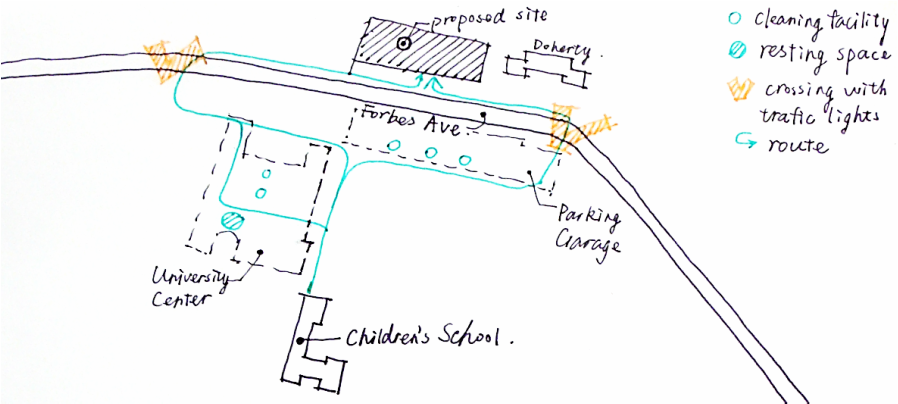
\includegraphics[width=\linewidth]{bridge1.png}
  \caption{Detouring Path from Children's School to the Proposed Site}
  \label{fig:bridge1}
\end{subfigure}
\begin{subfigure}{0.7\textwidth}
  \centering
  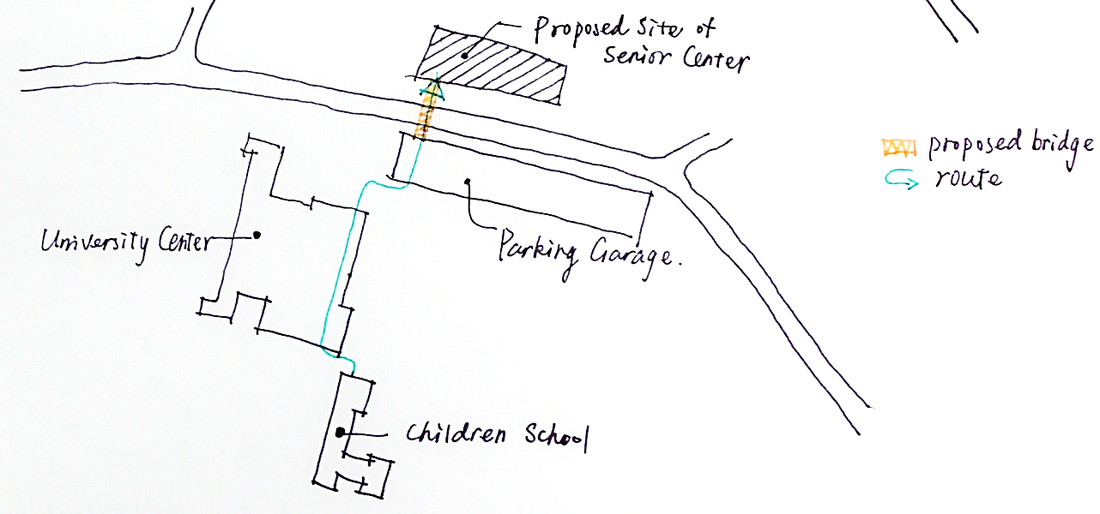
\includegraphics[width=\linewidth]{bridge2.png}
  \caption{Creating a Bridge to Reduce Detouring Distance}
  \label{fig:bridge2}
\end{subfigure}
\caption{Bridge Connecting Parking Garage and Senior Center}
\label{fig:bridge}
\end{figure}

\begin{figure}
\centering
\begin{subfigure}{\textwidth}
  \centering
  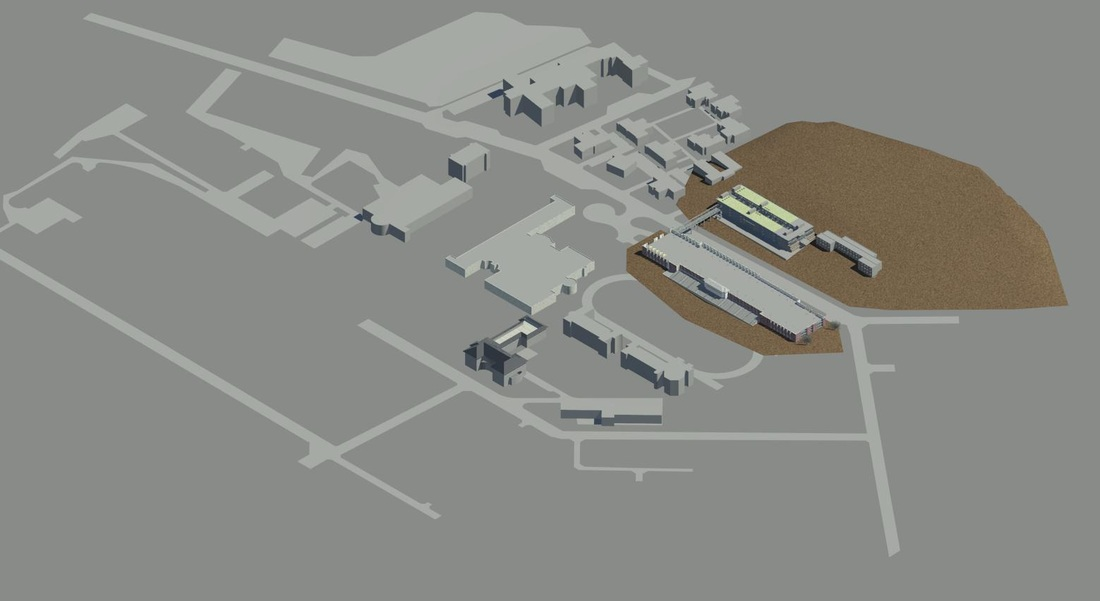
\includegraphics[width=0.9\textwidth]{site.jpg}
  \caption[Site Planning]{Site Planning Perspective View}
  \label{fig:site}
\end{subfigure}
\begin{subfigure}{\textwidth}
  \centering
  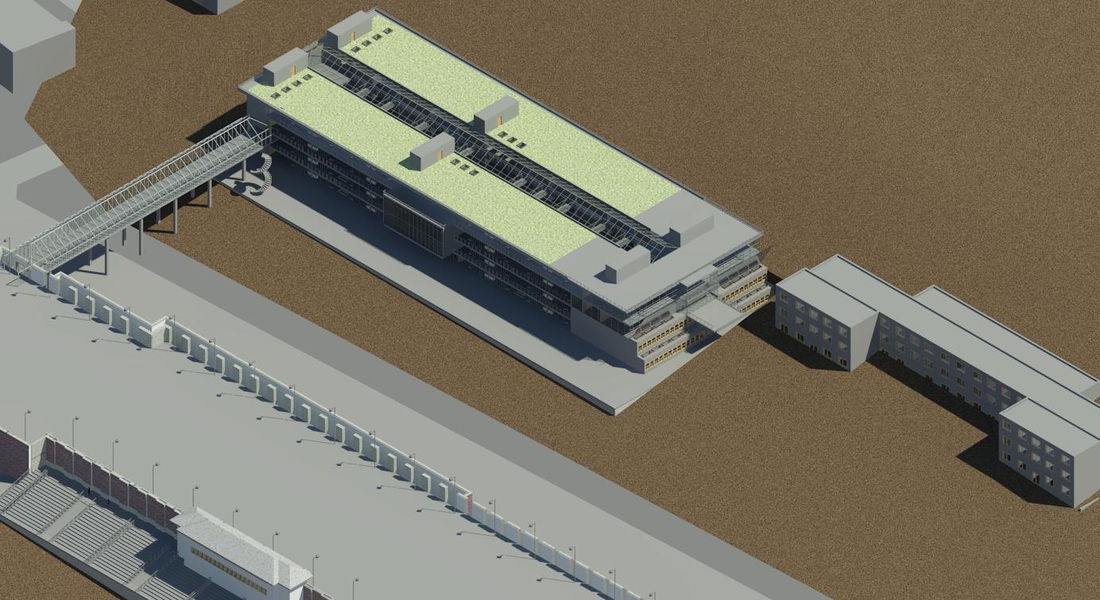
\includegraphics[width=0.9\textwidth]{siteClose.jpg}
  \caption[Site Planning Closer View]{Site Planning Closer View}
  \label{fig:siteClose}
\end{subfigure}
\caption{Site Planning}
\label{fig:siteAll}
\end{figure}
\section{Living Unit and Group Design}
\subsection{Topological Pattern of Living Cluster Design}
There are two aspects of aging: the ``biological process'' and the
``social passage''. For the social passage, as one become aged, one
tends to encounter a dramatic change in the social roles, some tends
to withdraw from previous responsibilities, some seeks to engagement
in new social roles~\cite{Perkins2004}. Providing a soft transition
and a variety of choices is a key to maintain a balance between the
social connection and the degree of privacy. Upon this concern, the
basic space structure of public-private-transition is defined
recursively as follows.

Another reason to organize space in this pattern is to encourage a
group-assist living pattern, to encourage residents to give and
receive help from their neighbors and the living group, which can both
provide a sense of self-achievement for helping others, to prolong
the time of transferring to a higher nursing degree and to strengthen
bounds between residents.

Another concern is especially for higher degree of living care, the
varied degree layout facilitates privacy in care-giving and
receiving with small nursing group.

Yet another consideration is to assign each group a common space and
encourage the residents to arrange the decoration and space
functionality, which increases the sense of belonging.
\begin{figure}
\centering
\begin{subfigure}{0.7\textwidth}
  \centering
  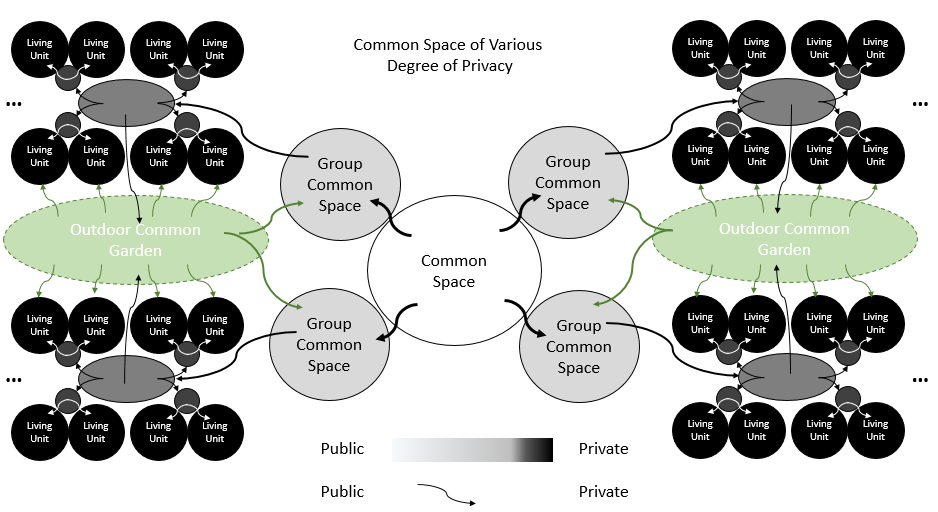
\includegraphics[width=\linewidth]{spacePattern.png}
  \caption{Space Pattern: Soft Transition of Public and Private Space}
  \label{fig:spacePattern}
\end{subfigure}
\begin{subfigure}{0.7\textwidth}
  \centering
  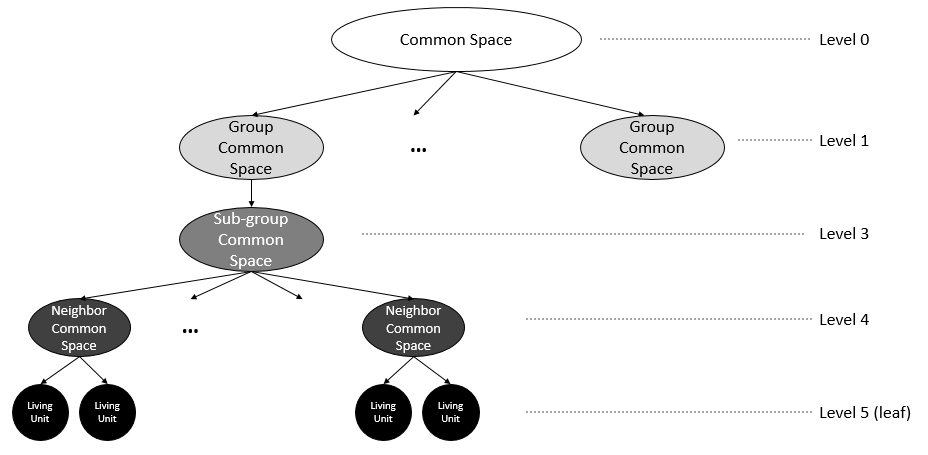
\includegraphics[width=\linewidth]{spaceTree.png}
  \caption{Tree Representation of Degree of Privacy Level}
  \label{fig:spaceTree}
\end{subfigure}
\caption{Space Pattern of Privacy Level Transition}
\label{fig:spacePrivacy}
\end{figure}
\subsection{Design Living Unit}~
\begin{figure}[htbp]
	\centering
		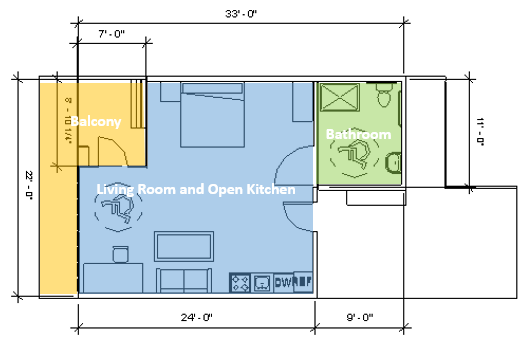
\includegraphics[width=0.7\textwidth]{plan1unit.png}
	\caption[Plan of Living Unit]{Plan of Living Unit}
	\label{fig:plan1unit}
\end{figure}
\begin{figure}[htbp]
	\centering
		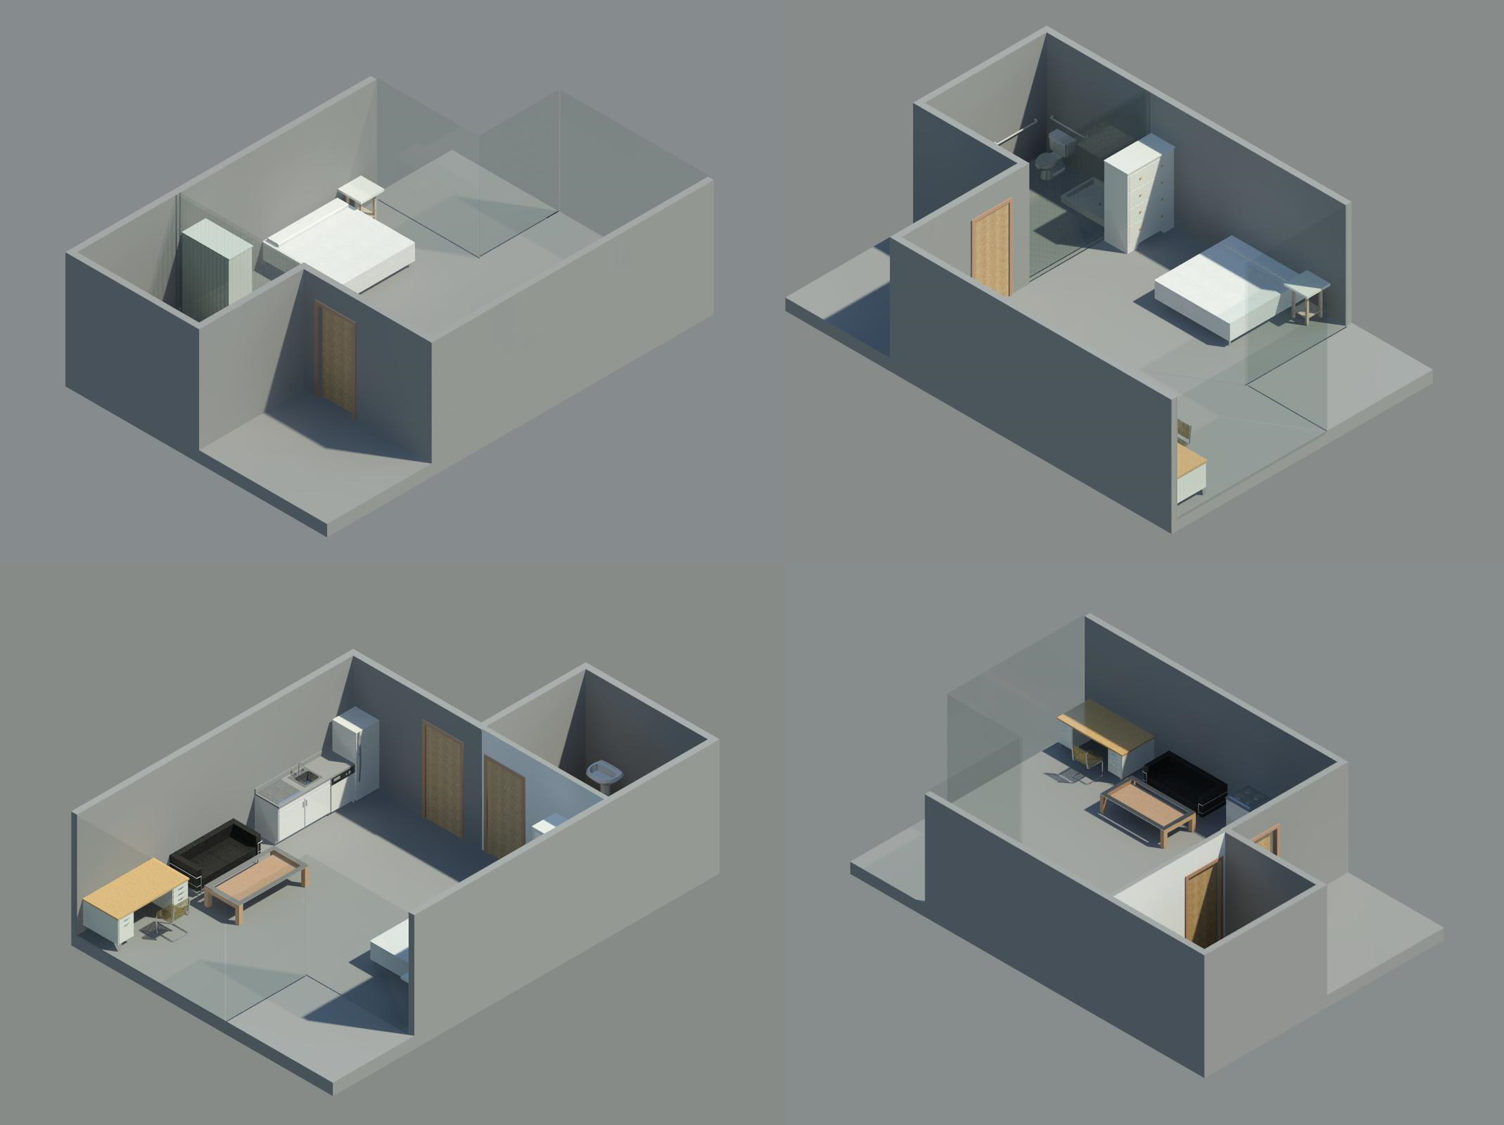
\includegraphics[width=\textwidth]{persUnit.png}
	\caption[Perspective View of Living Unit]{Perspective View of Living Unit}
	\label{fig:persUnit}
\end{figure}
\subsection{Living Unit Group and Common Space Design}
\begin{figure}[htbp]
	\centering
		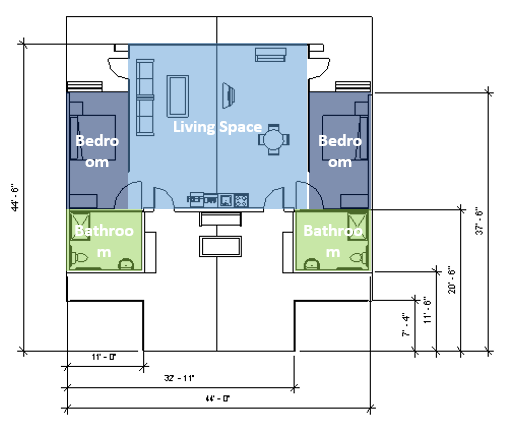
\includegraphics[width=0.7\textwidth]{plan2unit.png}
	\caption[Plan of Two-Unit Group]{Plan of Two-Unit Group}
	\label{fig:plan2unit}
\end{figure}
\begin{figure}[htbp]
	\centering
		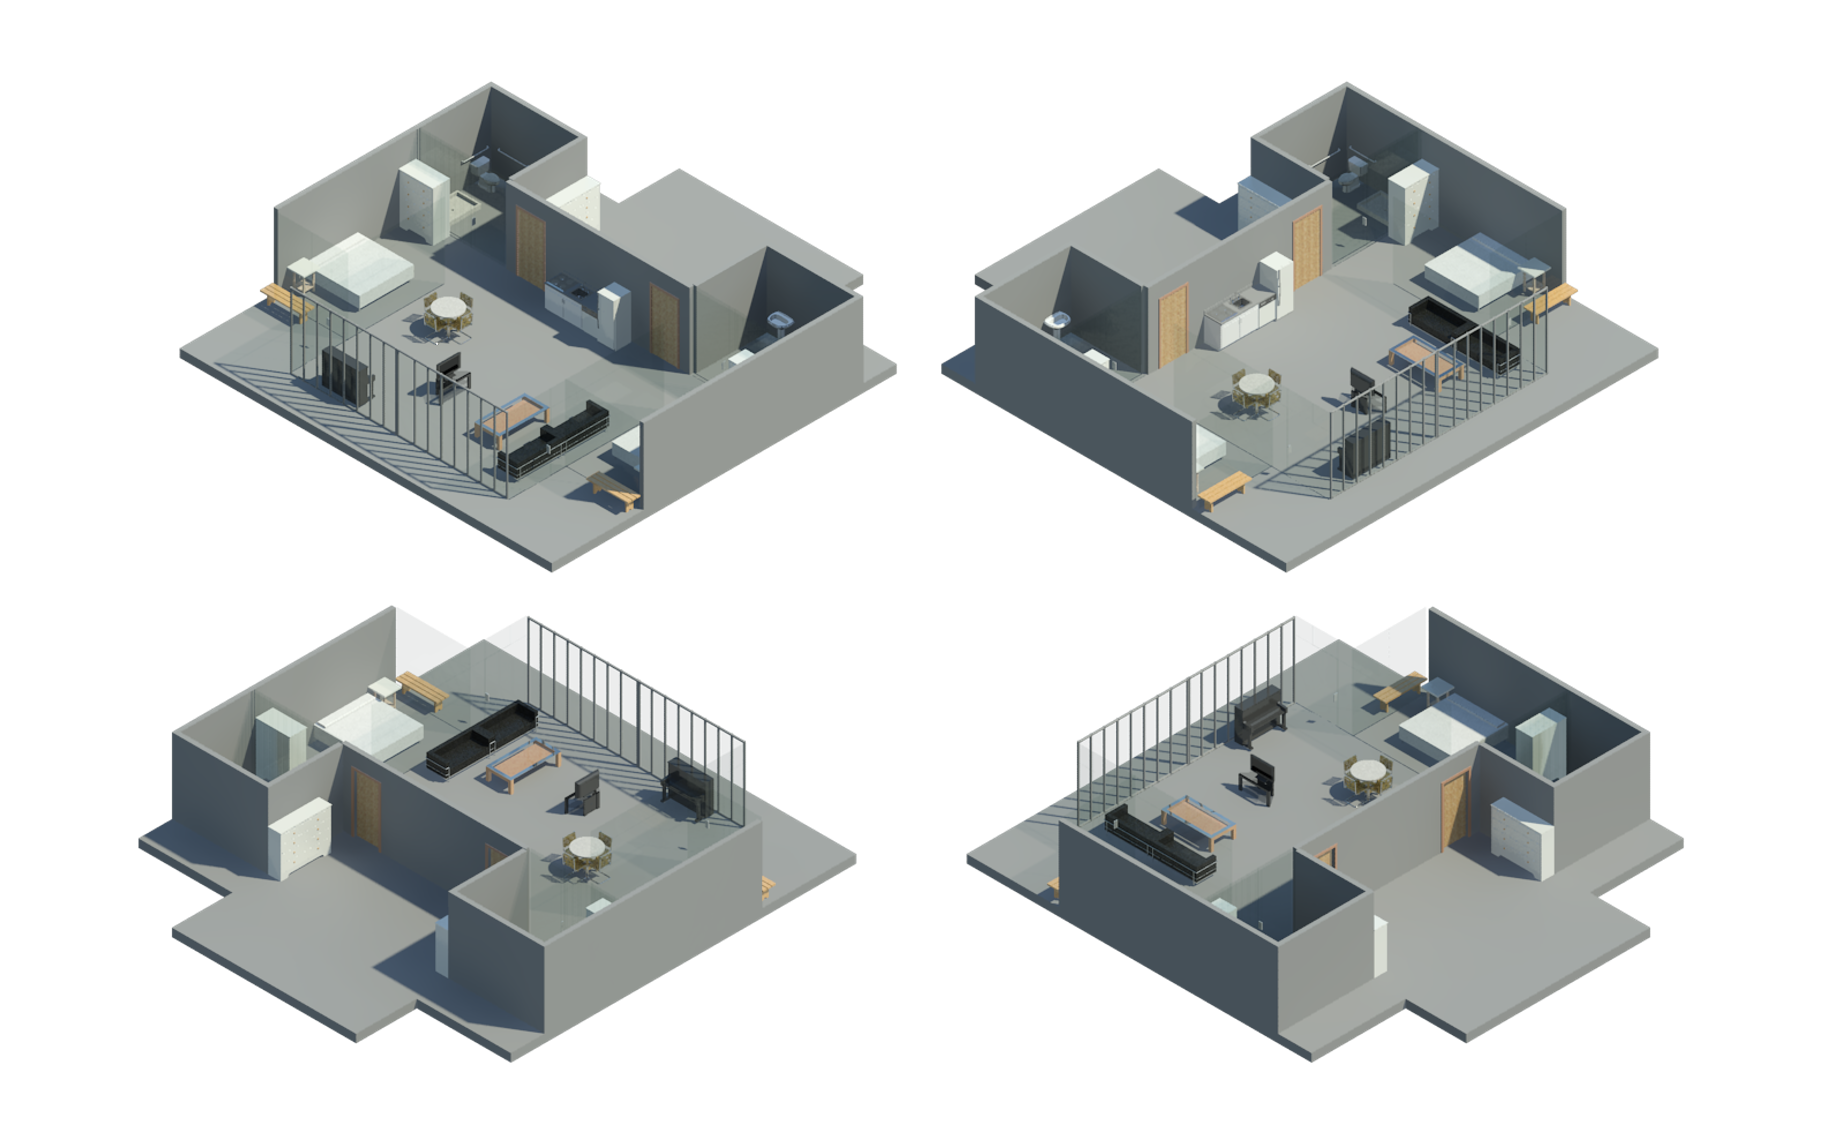
\includegraphics[width=\textwidth]{pers2unit.png}
	\caption[Perspective View of Two-Unit Group]{Perspective View of Two-Unit Group}
	\label{fig:pers2unit}
\end{figure}
\begin{figure}
\centering
\begin{subfigure}{\textwidth}
  \centering
  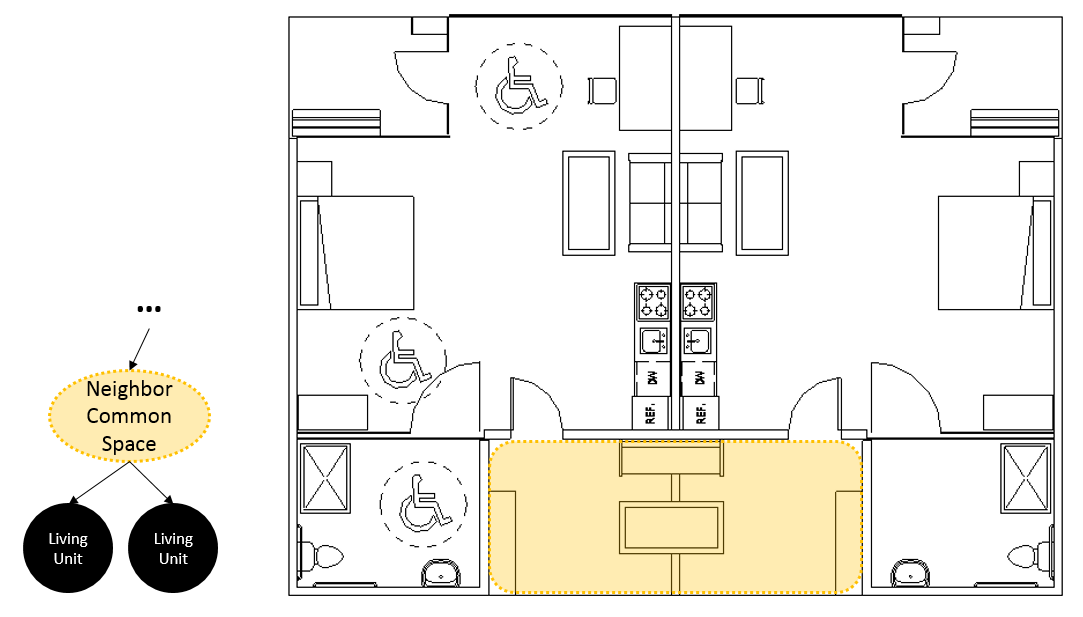
\includegraphics[width=\linewidth]{twoUnit-1.png}
  \caption{Common Space of Two Unit: Common Entrance}
  \label{fig:twoUnit-1}
\end{subfigure}
\begin{subfigure}{\textwidth}
  \centering
  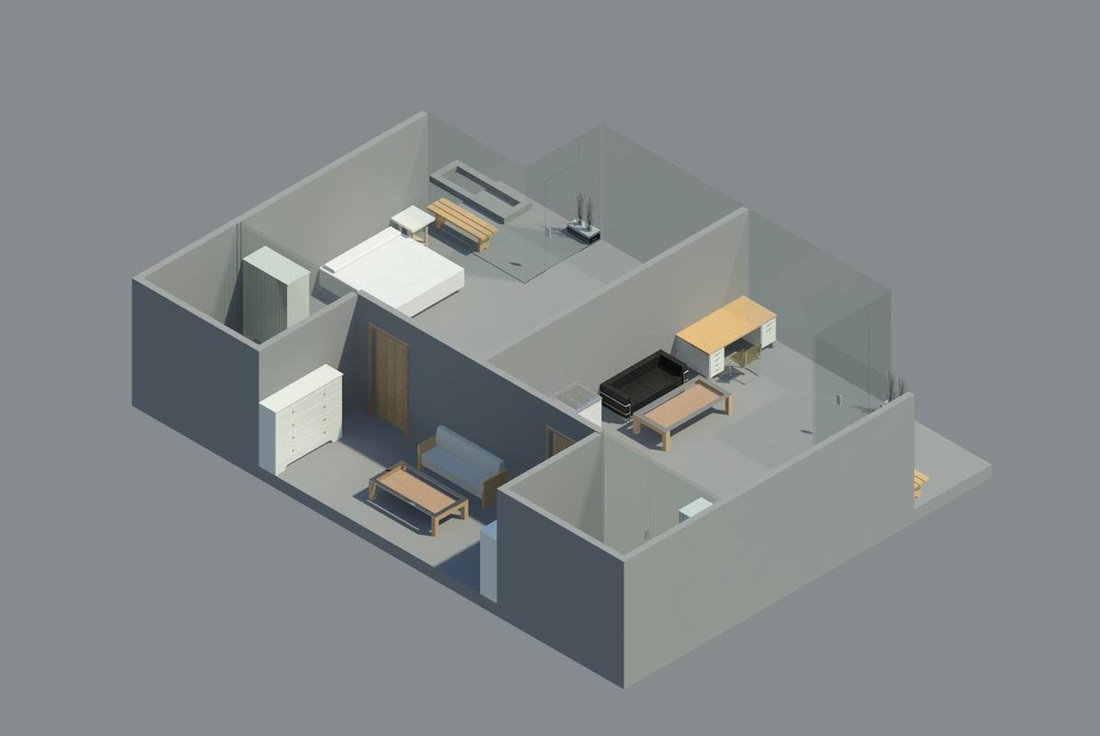
\includegraphics[width=\linewidth]{twoUnit-entrance.jpg}
  \caption{Perspective View of Common Space of Two Unit: Common Entrance}
  \label{fig:twoUnit-entrance}
\end{subfigure}
\caption{Two Unit Common Space}
\label{fig:twoUnitCommonSpaceEntrance}
\end{figure}

\begin{figure}
\centering
\begin{subfigure}{\textwidth}
  \centering
  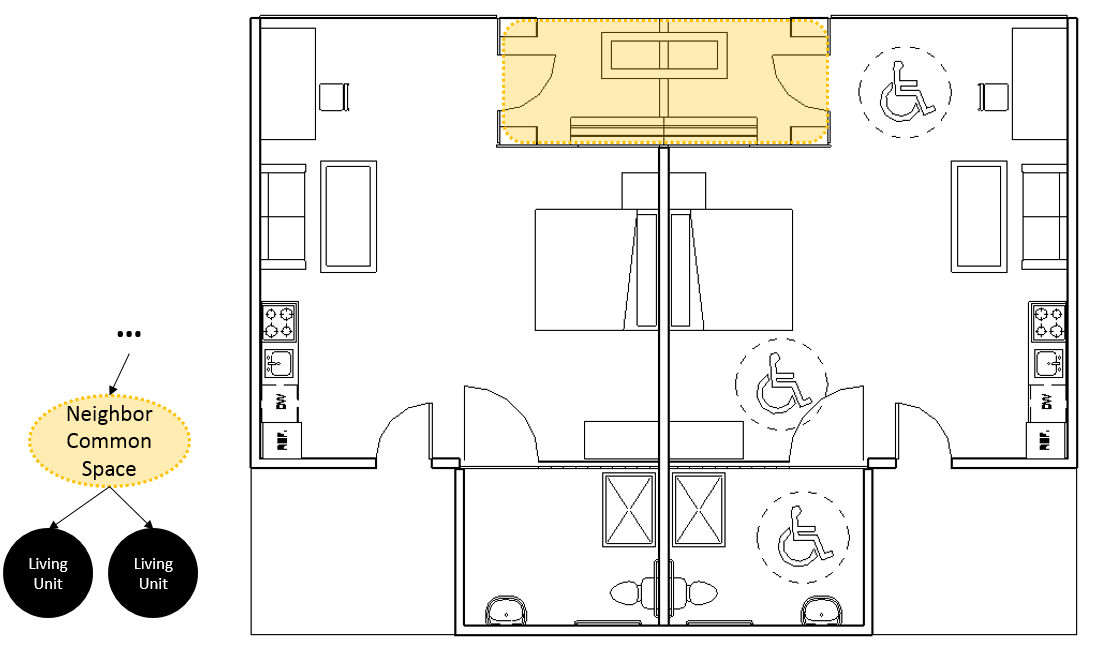
\includegraphics[width=\linewidth]{twoUnit-2.png}
  \caption{Common Space of Two Unit: Common Garden}
  \label{fig:twoUnit-2}
\end{subfigure}
\begin{subfigure}{\textwidth}
  \centering
  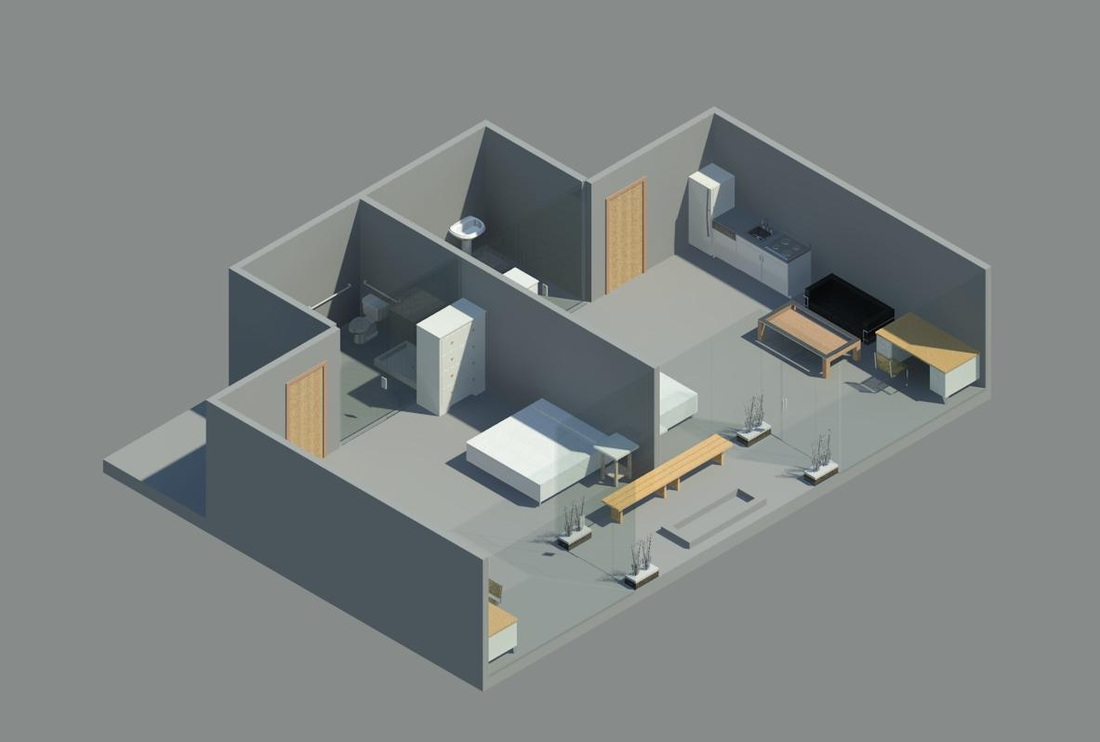
\includegraphics[width=\linewidth]{twoUnit-gd.jpg}
  \caption{Perspective View of Common Space of Two Unit: Common Garden}
  \label{fig:twoUnit-garden}
\end{subfigure}
\caption{Two Unit Common Space}
\label{fig:twoUnitCommonSpaceGarden}
\end{figure}

\begin{figure}
\centering
\begin{subfigure}{\textwidth}
  \centering
  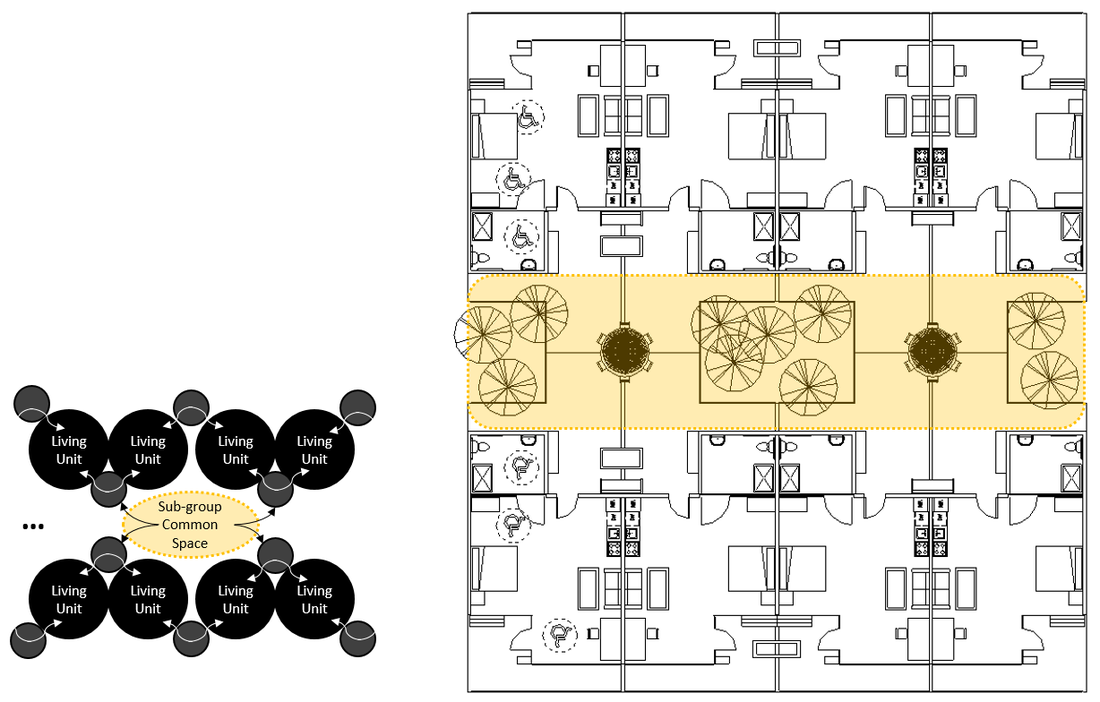
\includegraphics[width=\linewidth]{commonSpace8.png}
  \caption{Common Space of Eight Unit}
  \label{fig:commonSpace8}
\end{subfigure}
\begin{subfigure}{\textwidth}
  \centering
  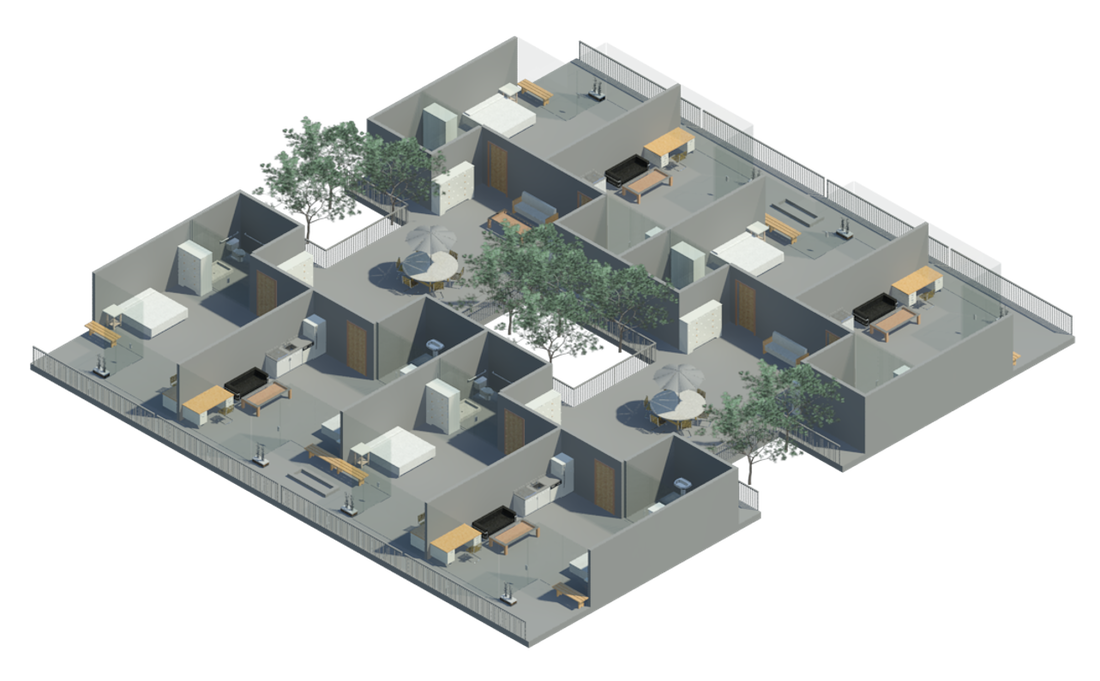
\includegraphics[width=\linewidth]{commonSpace8pers.png}
  \caption{Perspective View of Common Space of Eight Unit}
  \label{fig:commonSpace8pers}
\end{subfigure}
\caption{Eight Unit Common Space}
\label{fig:eightUnitCommonSpace}
\end{figure}

\begin{figure}
\centering
\begin{subfigure}{\textwidth}
  \centering
  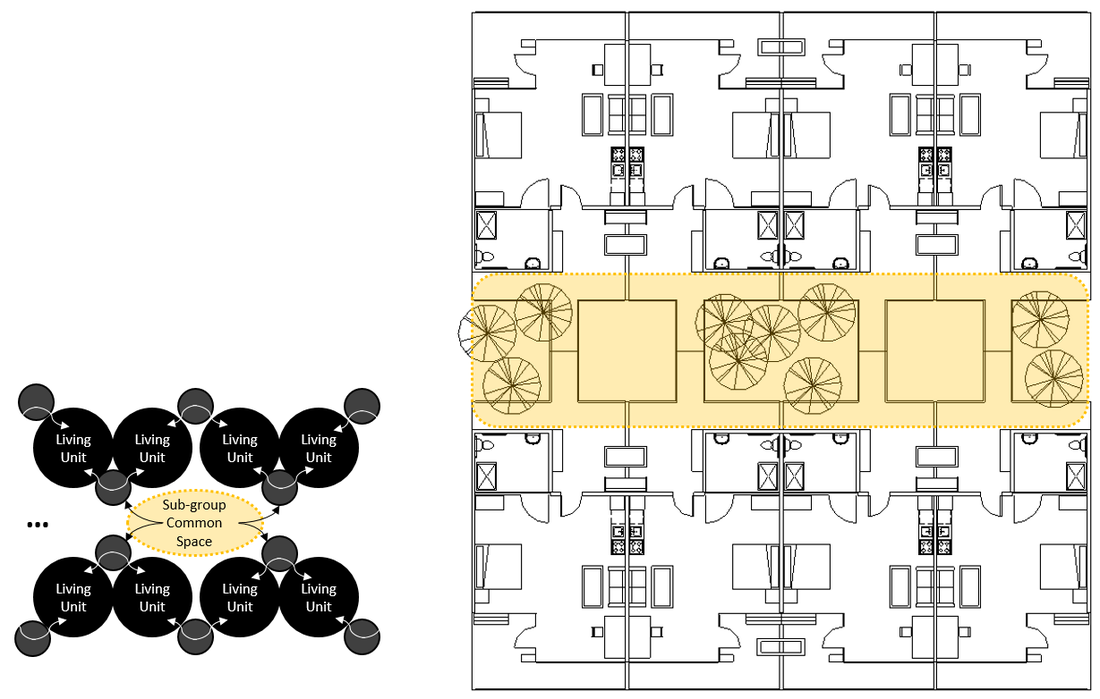
\includegraphics[width=\linewidth]{commonSpace8up.png}
  \caption{Common Space of Eight Unit: Upper Level}
  \label{fig:commonSpace8}
\end{subfigure}
\begin{subfigure}{\textwidth}
  \centering
  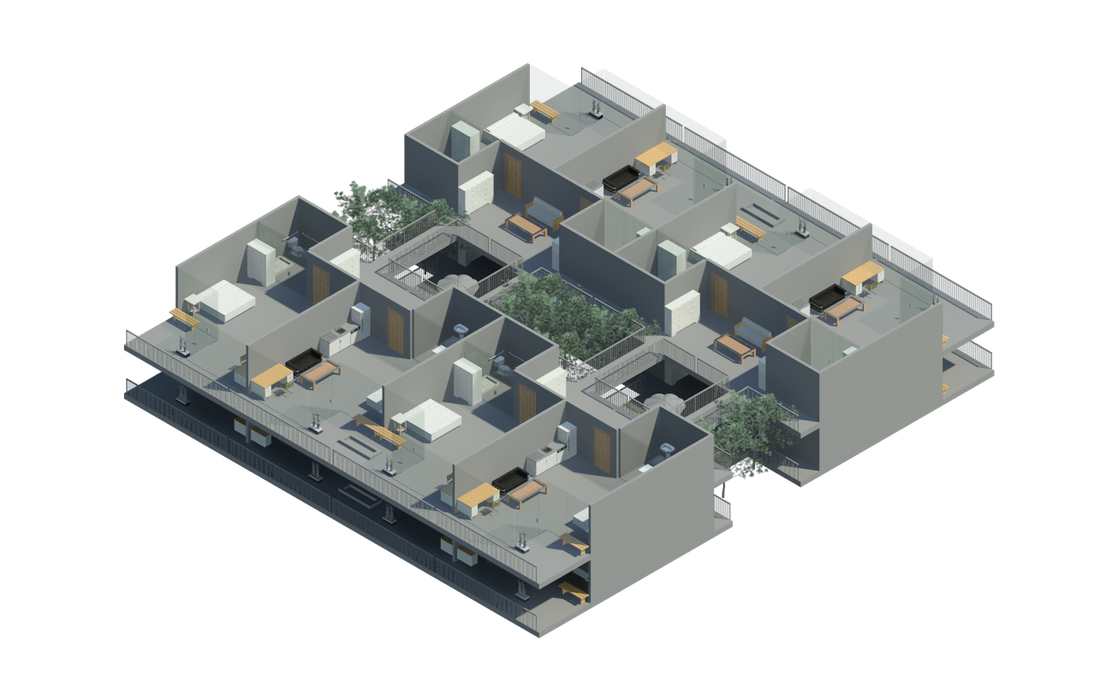
\includegraphics[width=\linewidth]{commonSpace8upPers.png}
  \caption{Perspective View of Common Space of Eight Unit: Upper Level}
  \label{fig:commonSpace8pers}
\end{subfigure}
\caption{Eight Unit Common Space: Upper Level}
\label{fig:eightUnitCommonSpaceUp}
\end{figure}

\newpage
\section{Path Arrangement}~
The major concern for path design includes:
\begin{itemize}
\item To create more chance of encountering people, both the elderly residents and the young people.
\item To accommodate the needs for the Alzheimer Disease victims. \\A ``wandering loop'' (\fref{fig:path}) is needed to accomodate the behavior change for the Alzheimer Disease victims. For more detailed information, please refer to the case study in \cref{Chapter3}
\end{itemize}

\begin{figure}[htbp]
	\centering
		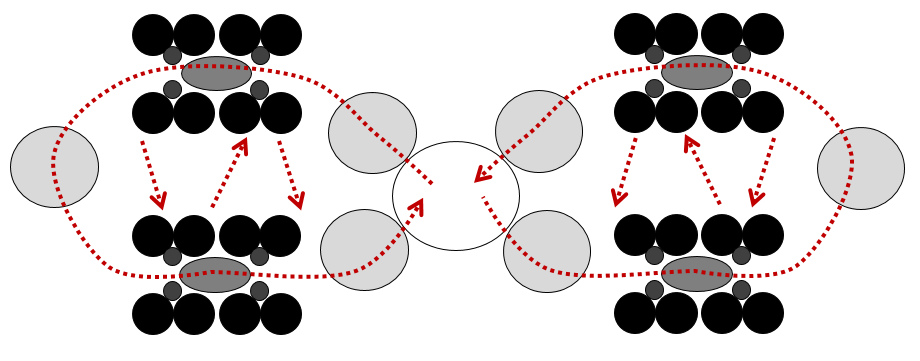
\includegraphics[width=0.7\textwidth]{path.png}
	\caption[Path Pattern]{Path Pattern}
	\label{fig:path}
\end{figure}
\subsection{Access to Nature}
In order to allow for easy access to nature, the indoor garden is created between each of the two major row of living units, allowing for access to nature in the indoor environment~\fref{fig:indoorGarden}.
\begin{figure}[htbp]
	\centering
		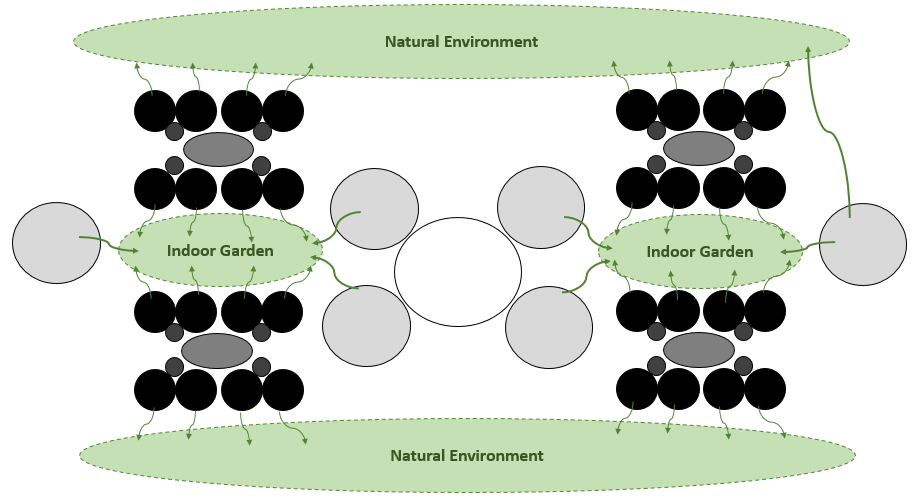
\includegraphics[width=0.7\textwidth]{indoorGarden.png}
	\caption[Access to Nature]{Access to Nature}
	\label{fig:indoorGarden}
\end{figure}
\subsection{Easier Way Finding}
\section{Sustainable System}
The components involved in the sustainable system include roof gardens, rooftop pv system, green facade, rain collecting system and food production chain resulted from the gardening. A draft system integration diagram is shown in \fref{fig:sketchSustainable}
\begin{figure}[htbp]
	\centering
		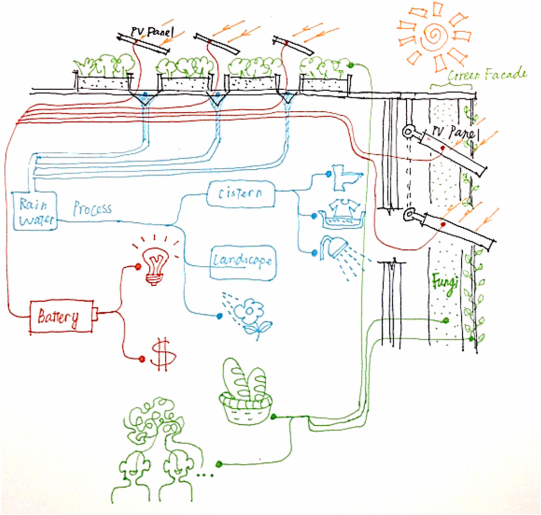
\includegraphics[width=0.8\textwidth]{sketchSustainable.png}
	\caption[System Integration Draft Diagram]{System Integration Draft Diagram}
	\label{fig:sketchSustainable}
\end{figure}